\subsection{Anomaly-Aware LSTMD}
\label{sec:lstmd_results}

The same question was asked of the probabilistic LSTM. We trained LSTMD with raw inputs and with anomaly-aware inputs on the same eleven traces, using the same chronological split as the HBNN (64\% training, 16\% validation, 20\% test) and the Gaussian negative log-likelihood, so the asymmetric loss is not used here. Each model was trained for up to 500 epochs with the best validation weights restored, and both variants reuse the same tuned hyperparameter sets released with the reference implementation, chosen per configuration and trace. The upper bound at target level $\gamma$ is the predicted mean plus $z_\gamma$ times the predicted standard deviation, so it reflects aleatoric uncertainty only. One run was made per configuration, trace, and variant (72 fits: 36 raw and 36 anomaly-aware; the univariate models are trained separately for CPU and memory), so there is no seed-to-seed spread and the numbers below are descriptive. \todo{Confirm the LSTMD anomaly input channels, the loss, and the spike label (about 11\% of test points are labelled as spikes).}

\textit{Point accuracy.}
Table~\ref{tab:lstmd_acc} and Fig.~\ref{fig:lstmd_summary}(a) give the point-forecast results. In the multi-trace configurations the anomaly inputs change little. The paired MSE ratio, anomaly-aware over raw, is 1.002 for M-U and 0.993 for M-B, the MAE ratios are 1.003 and 0.999, and the anomaly-aware model is better on 7 and 5 of the 11 traces respectively. The single-trace configurations are worse or mixed. S-B gets worse (MSE ratio 1.104, a bootstrap over traces gives a 95\% interval of 1.02--1.21, and only 4 of 11 traces improve), and S-U is worse for CPU (1.075) and about unchanged for memory (0.986). The large drop in S-U memory MSE in Table~\ref{tab:lstmd_acc} (0.0046 to 0.0030) is not an effect of the inputs. It comes from one trace, gc19\_e, where the raw memory model failed (see the reproduction above) and the anomaly-aware one did not. The anomaly inputs therefore do not give LSTMD a consistent accuracy gain.

\textit{Spikes.}
Fig.~\ref{fig:lstmd_summary}(a) and the right half of Table~\ref{tab:lstmd_acc} look at the spike points. The effects are small and mixed. Spike MSE is about 4\% lower for M-U on both resources and 19\% lower for M-B memory, but 6\% higher for M-B CPU, and the single-trace models move by 5\% or less. In the multi-trace models the mean forecast lies below the actual value at about 99\% of spike points with and without the anomaly inputs. As with the HBNN, the network gets closer to the spike but almost always still lands under it. The overall underprediction rate of M-B does fall, from 53.7\% to 48.4\% of points, but that shift does not reach the spikes.

\textit{Service level.}
Table~\ref{tab:lstmd_service} and Fig.~\ref{fig:lstmd_summary}(b,c) show the upper bound. For the multi-trace models and S-B, coverage and cost are nearly identical with and without the anomaly inputs. At the 95\% target the multi-trace models reach an SR of about 95\% at a TPR of 113--115\%, and at the 99\% target about 98.2\% at 120--121\%. The inputs make calibration slightly worse, not better: the mean gap grows from 0.69 to 1.48 percentage points for M-B and from 0.61 to 0.99 for M-U. In every configuration the realised SR is above the target at the low levels and falls short at the highest ones (98.2\% at the 99\% target). For S-U the raw model needs a TPR of 121.7\% at the 95\% target against 113.4\% for the anomaly-aware one. This is again the failed gc19\_e memory fit, whose very large predicted variance inflates the bound (TPR of 290\%). Without that series the two are 113.7\% and 113.4\%, and the raw SR is 0.9 points higher.

Both probabilistic models used the same split, so one comparison is worth making. The raw multi-trace LSTMD already reaches an SR of 95.1\% at a TPR of 114.8\% for M-B, close to the anomaly-aware HBNN (95.8\% at 116.4\%) and much more efficient than the raw HBNN (93.7\% at 129.4\%). The HBNN used one shared, untuned hyperparameter set while LSTMD used the tuned sets from the reference, so this is not a clean architecture comparison. It is consistent with reading part of the HBNN gain from the anomaly inputs as the repair of a weak raw baseline.

\begin{table*}[!t]
\caption{LSTMD with and without anomaly-aware inputs, mean over 11 traces (one run per trace). Spike under-prediction is the share of spike points where the mean forecast lies below the actual demand. Lower is better in every column; the better value of each pair is in bold.}
\label{tab:lstmd_acc}
\centering
\footnotesize
\setlength{\tabcolsep}{4.5pt}
\begin{tabular}{llcccccccc}
\toprule
 & & \multicolumn{2}{c}{MSE} & \multicolumn{2}{c}{MAE} & \multicolumn{2}{c}{Spike MSE} & \multicolumn{2}{c}{Spike under-pred. (\%)}\\
\cmidrule(lr){3-4}\cmidrule(lr){5-6}\cmidrule(lr){7-8}\cmidrule(lr){9-10}
Config. & Res. & Raw & Anomaly & Raw & Anomaly & Raw & Anomaly & Raw & Anomaly\\
\midrule
S-U & CPU & \textbf{0.0032} & 0.0035 & \textbf{0.040} & 0.042 & \textbf{0.0103} & 0.0106 & 99.5 & \textbf{98.8}\\
 & Mem. & 0.0046 & \textbf{0.0030} & 0.046 & \textbf{0.036} & 0.0099 & \textbf{0.0090} & \textbf{90.4} & 99.1\\
\addlinespace[2pt]
S-B & CPU & \textbf{0.0032} & 0.0036 & \textbf{0.040} & 0.043 & 0.0089 & \textbf{0.0086} & 97.1 & \textbf{94.7}\\
 & Mem. & \textbf{0.0032} & 0.0036 & \textbf{0.037} & 0.040 & \textbf{0.0088} & 0.0092 & 97.5 & 97.5\\
\addlinespace[2pt]
M-U & CPU & 0.0031 & 0.0031 & 0.039 & 0.039 & 0.0119 & \textbf{0.0112} & 99.6 & \textbf{99.5}\\
 & Mem. & 0.0030 & \textbf{0.0029} & 0.035 & 0.035 & 0.0096 & \textbf{0.0094} & \textbf{99.0} & 99.2\\
\addlinespace[2pt]
M-B & CPU & 0.0031 & \textbf{0.0030} & 0.039 & 0.039 & \textbf{0.0099} & 0.0104 & \textbf{98.2} & 98.8\\
 & Mem. & 0.0030 & 0.0030 & 0.036 & 0.036 & 0.0094 & \textbf{0.0080} & \textbf{98.7} & 98.9\\
\bottomrule
\end{tabular}
\end{table*}

\begin{figure*}[!t]
\centering
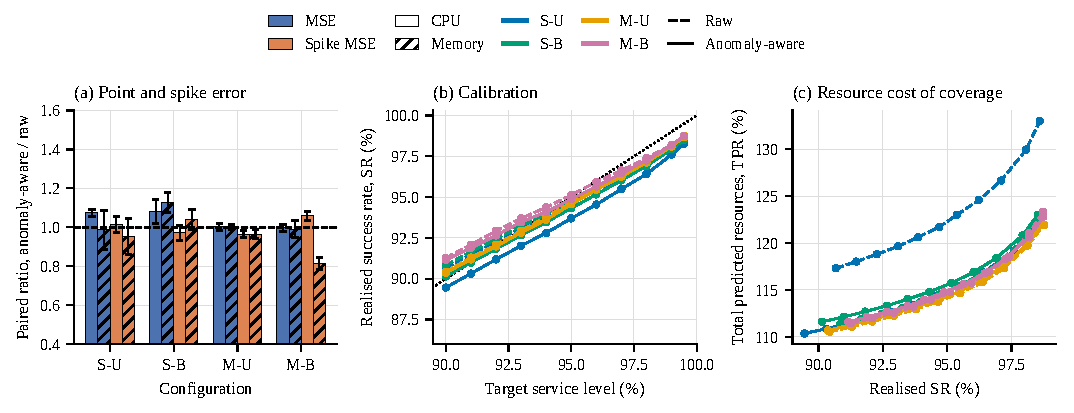
\includegraphics[width=\textwidth]{lstmd_fig_summary.pdf}
\caption{LSTMD with raw and anomaly-aware inputs. (a) Paired ratio of overall MSE and spike MSE, anomaly-aware over raw, for CPU and memory; values below one favour the anomaly-aware inputs, and error bars show the standard error over 11 traces. (b) Realised success rate against the target service level, averaged over CPU and memory; the dotted diagonal is perfect calibration. (c) Total predicted resources against realised SR. Dashed lines are raw inputs and solid lines anomaly-aware inputs.}
\label{fig:lstmd_summary}
\end{figure*}

\begin{table}[!t]\caption{Service-level behaviour of the LSTMD upper bound (mean over CPU, memory and 11 traces, one run per trace). SR is the realised success rate, TPR the total predicted resources as a percentage of actual demand, and Cal.\ the mean absolute gap between realised and target SR over the eleven target levels from 90\% to 99.5\%.}
\label{tab:lstmd_service}
\centering
\footnotesize
\setlength{\tabcolsep}{3.6pt}
\begin{tabular}{llccccc}
\toprule
 & & \multicolumn{2}{c}{95\% target} & \multicolumn{2}{c}{99\% target} & Cal.\\
\cmidrule(lr){3-4}\cmidrule(lr){5-6}
Config. & Input & SR & TPR & SR & TPR & (pp)\\
\midrule
S-U & Raw & 94.7 & 121.7 & 98.1 & 130.0 & 1.06\\
 & Anomaly & 93.7 & 113.4 & 97.6 & 119.2 & 1.21\\
\addlinespace[2pt]
S-B & Raw & 94.7 & 114.5 & 98.0 & 120.5 & 0.62\\
 & Anomaly & 94.3 & 114.8 & 97.9 & 120.8 & 0.70\\
\addlinespace[2pt]
M-U & Raw & 94.7 & 113.7 & 98.1 & 119.7 & 0.61\\
 & Anomaly & 94.6 & 113.9 & 98.1 & 119.8 & 0.99\\
\addlinespace[2pt]
M-B & Raw & 95.1 & 114.8 & 98.2 & 121.1 & 0.69\\
 & Anomaly & 94.9 & 114.7 & 98.2 & 120.6 & 1.48\\
\bottomrule
\end{tabular}
\end{table}

